\chapter{ROS Programming with Python}
\label{cprog}


\section{Overview}
ROS is an open-source, meta-operating system for your robot. It provides the services you would expect from an operating system, including
hardware abstraction, low-level device control, implementation of commonly-used functionality, message-passing between processes, and package
management. It also provides tools and libraries for obtaining, building, writing, and running code across multiple computers. \\

\begin{itemize}
\item The ROS runtime ``graph" is a peer-to-peer network of processes (potentially distributed across machines) that are loosely coupled
using the ROS communication infrastructure. ROS implements several different styles of communication, including synchronous RPC-style
communication over services, asynchronous streaming of data over topics, and storage of data on a Parameter Server. \\

\item For more details about ROS: \url{http://wiki.ros.org/}
\item How to install on your own Ubuntu: \url{http://wiki.ros.org/ROS/Installation}
\item For detailed tutorials: \url{http://wiki.ros.org/ROS/Tutorials}
\item ``\textit{A Gentle Introduction to ROS}", Chapter 2 and 3. \url{http://coecsl.ece.illinois.edu/ece470/agitr-letter.pdf}
\end{itemize}

\section{ROS Concepts}
The basic concepts of ROS are nodes, Master, messages, topics, Parameter Server, services, and bags. However, in this course, we will only
be encountering the first four.
\begin{itemize}
\item \texttt{Nodes}  “programs” or ”processes” in ROS that perform computation. For example, one node controls a laser range-finder, one node controls
 he wheel motors, one node performs localization ...
\item \texttt{Master} Enable nodes to locate one another, provides parameter server, tracks publishers and subscribers to topics, services.
In order to start ROS, open a terminal and type:
\begin{lstlisting}[language=bash]
$ roscore
\end{lstlisting}
roscore can also be started automatically when using roslaunch in terminal, for example:
\begin{lstlisting}[language=bash]
$ roslaunch <package name> <launch file name>.launch
# the launch file for all our labs:
$ roslaunch ur_robot_driver ur3e_bringup.launch 
\end{lstlisting}
\item \texttt{Messages} Nodes communicate with each other via messages.  A message is simply a data structure, comprising typed fields.
\item \texttt{Topics} Each node publish/subscribe message topics via send/receive messages. A node sends out a message by publishing it to a
given topic. There may be multiple concurrent publishers and subscribers for a single topic, and a single node may publish and/or subscribe to 
multiple topics.In general, publishers and subscribers are not aware of each others' existence.
\end{itemize}
\begin{figure}[h]
	\centering
		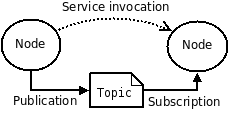
\includegraphics[scale=0.6]{image/appendixA_ROS_basic_concepts.png}
	\caption{\figlbl{ros_concept} source: \url{http://wiki.ros.org/ROS/Concepts}}
\end{figure}

\section{Before we start..}
Here are some useful Linux/ROS commands
\begin{itemize}
\item The command “ls” stands for (List Directory Contents), List the contents of the folder, be it file or folder, from which it runs.
\begin{lstlisting}[language=bash]
$ ls
\end{lstlisting}

\item The “mkdir” (Make directory) command create a new directory with name path. However is the directory already exists, it will return an
error message “cannot create folder, folder already exists”.
\begin{lstlisting}[language=bash]
$ mkdir <new_directory_name>
\end{lstlisting}

\item The command “pwd” (print working directory), prints the current working directory with full path name from terminal
\begin{lstlisting}[language=bash]
$ pwd
\end{lstlisting}

\item The frequently used “cd” command stands for change directory. 
\begin{lstlisting}[language=bash]
$ cd /home/user/Desktop
\end{lstlisting}
return to previous directory
\begin{lstlisting}[language=bash]
$ cd ..
\end{lstlisting}
Change to home directory
\begin{lstlisting}[language=bash]
$ cd ~
\end{lstlisting}

\item The hot key ``ctrl+c" in command line \textbf{terminates} current running executable.  If ``ctrl+c" does not work, closing your terminal as that will also end the running Python program. \textbf{DO NOT USE ``ctrl+z" as it can leave some unknown applications running in the background}.   

\item If you want to know the location of any specific ROS package/executable from in your system, you can use ``rospack" find  ``package name" command. For 
example, if you would like to find `lab2pkg\_py' package, you can type in your console
\begin{lstlisting}[language=bash]
$ rospack find lab2pkg_py
\end{lstlisting}

\item To move directly to the directory of a ROS package, use roscd. For example, go to lab2pkg\_py package directory
\begin{lstlisting}[language=bash]
$ roscd lab2pkg_py
\end{lstlisting}

\item Display Message data structure definitions with rosmsg
\begin{lstlisting}[language=bash]
# Display the fields in the msg
$ rosmsg show <message_type>
\end{lstlisting}

\item rostopic, A tool for displaying debug information about ROS topics,
including publishers, subscribers, publishing rate, and
messages.
\begin{lstlisting}[language=bash]
# Print messages to screen
$ rostopic echo /topic_name
# List all the topics available
$ rostopic list
# Publish data to topic
$ rostopic pub <topic-name> <topic-type> [data...]  
\end{lstlisting}
\end{itemize}

\section{Create your own workspace}
Since other groups will be working on your same computer, you should backup your code to a USB drive or cloud drive everytime you come to lab.  This way if 
your code is tampered with (probably by accident) you will have a backup.
\begin{itemize}
\item Log on to the computer as `rvc' with the password `123456'.  If you log on as `guest', you will not be able to use ROS.
\item First create a folder in the home directory, mkdir catkin\_(yourNETID).  It is not required to have "catkin" in the folder name but it is recommended.
\begin{lstlisting}[language=bash]
$ mkdir -p catkin_(yourID)/src
$ cd catkin_(yourID)/src
$ catkin_init_workspace
\end{lstlisting}
\item Even though the workspace is empty (there are no packages in the 'src' folder, just a single CMakeLists.txt link) you can still "build" the 
workspace. Just for practice, build the workspace.
\begin{lstlisting}[language=bash]
$ cd ~/catkin_(yourID)/
$ catkin_make
\end{lstlisting}
\item \textbf{VERY IMPORTANT}: Remember to \textbf{ALWAYS} source when you open a new command prompt, so you can utilize the full convenience of Tab completion in ROS.
Under workspace root directory:
\begin{lstlisting}[language=bash]
$ cd catkin_(yourID)
$ source devel/setup.bash
\end{lstlisting}
\end{itemize}

\section{Running a Node}
\begin{itemize}
\item Once you have your catkin folder initialized, add the UR3 driver and lab starter files.  The compressed file lab2andDanDriver.tar.gz, found
at the class website contains the driver code you will need for all the ECE 470 labs along with the starter code for LAB 2.  Future lab compressed 
files will only contain the new starter code for that lab.  Copy lab2andDriverPy.tar.gz to your catkin directories ``src" directory.  Change directory
to your ``src" folder and uncompress by typing ``tar -xvf lab2andDriver.tar.gz".  You can also do this via the GUI by double clicking on the compressed file and dragging the folders into the new location.

``cd .." back to your catkin\_(yourID) folder and build the code
with ``catkin\_make"
\item After compilation is complete, we can start running our own nodes. For example our lab2node node. However, before running any nodes, we must
have roscore running. This is taken care of by running a launch file.

\begin{lstlisting}[language=bash]
$ roslaunch ur_robot_driver ur3e_bringup.launch
\end{lstlisting}

This command runs both roscore and the UR3 driver that acts as a subscriber waiting for a command message that controls the UR3's motors.


\item Open a new command prompt with ``ctrl+shift+N", cd to your root workspace directory, and source it ``source devel/setup.bash".

\item We may also need to make lab2\_exec.py executable.
\begin{lstlisting}[language=bash]
$ chmod +x lab2_exec.py
\end{lstlisting}

\item Run your node with the command rosrun in the new command prompt. Example of running lab2node node in lab2pkg package: 
\begin{lstlisting}[language=bash]
$ rosrun ur3e_driver_ece470 ur3e_driver_ece470
# Another terminal
$ rosrun lab2pkg_py lab2_exec.py
\end{lstlisting}
\end{itemize}

% Note that the ``-{}-simulator True" tells it you are running on the simulator, while ``-{}-simulator False" tells the program you are running on real hardware.  This flag is currently only applicable to Lab 2.

\section{More Publisher and Subscriber Tutorial}
Please refer to the webpage: \url{http://wiki.ros.org/ROS/Tutorials/WritingPublisherSubscriber(c\%2B\%2B)}


